\section{Designing FSO Links for Flexible Inter-Rack Networking}
\label{sec:fso}

\samir{terminology question: FSO link, transceiver, device, device assembly, or system?? Among these device 
or system sound too generic and something a non-technical person would use. We can use link and
transceiver depending on context. They are also more common in networking lit.}

%% just say high level what to expect in this section
 In this section, we begin by specifying the design requirements for FSOs 
and highlight why existing FSO technologies fail to meet the  requirements that
the \ArchName vision imposes.  Then, we highlight a design roadmap for meeting
these requirements.


\subsection{Overview and Requirements}


%% what are the requirements
The design of FSO transceivers in \ArchName must 
 simultaneously meet the following requirements: 
\begin{packeditemize}
\item {\em Size, power, and cost effectiveness:}
Our  goal is to design a single FSO transceiver assembly (i.e., including
alignment and beam redirection machinery) will have $\approx$ 3"x8" footprint
so that a few tens of such devices can be packed on the ToR.  The power
consumption should be modest and they must be cost-competitive to existing
networks. 

\item {\em Ability to provide 10-100Gbps data rate:}  As DC traffic rates 
 are growing~\cite{ananta} and demands for  40~Gbps networks emerge,
 our design  must be capable of providing high throughput.

\item {\em Fast and precise alignment and steering :} \samir{terminology question: `steering' or `redirection' here??
note that SM is not technically steering. So we were looking for more a general word.
Redirection is a better word as then we can say switching for SM and steering for galvo.
Steering brings in the sense that it is continuous, but it does not need to be get to what we want.} For FSO links to provide
high throughput, the transmit/receive devices must be precisely aligned. Thus,
we need mechanisms for robust re-aligment in the presence of environmental
effects; e.g., vibrations, changes in airflow. Furthermore, to provide
fine-grained reconfigurability, we need to be able to steer the laser beams to
connect to another  FSO transceiver on another rack determined by the management layer in
Section~\ref{}.  
 
\end{packeditemize}

% existing solutions suck
 Unfortunately, existing FSO transceivers target  {\em fixed} terrestrial long
distance (miles) communication~\cite{} and  do not meet our size, power or cost
goals.  For example, a typical commercial system~\cite{lightpointe} is 2 cubic
feet, costs \$5-10K for a single link, consumes \plsfill watts. The reason for the 
significantly large numbers is that
they have to overcome  outdoor challenges --- beam path
variations due to a host of environmental factors~\cite{}, larger
transmit power requirements for longer distances; alignment problems due to structural swaying etc.  While
these issues largely disappear in the context of DCs and thus create a pathway for size, power,
and cost-optimized design, we have a  new requirement of fast reconfiguration. 



%%  what are our challenges
%This  requires us to rethink FSO design suitable for the \ArchName vision.  
 We outline the challenges and proposed approaches for FSO design in \ArchName
in a two-step process: (1) Designing the basic FSO link for a DC-scale
operation, and  (2) Fast and precise beam redirection to enable reconfiguration.  Our
research here  will inform the parameters (e.g., range, size, \red{cost}) which will
be input to the topology design problems  in Section~\ref{sec:topology}. 

\subsection{Cost-effective,  Small-Form Factor, and High Throughput FSO Links}

\begin{task}
We will design the FSO link including transmitter, receiver and the optical beam path for effective datacenter scale operation,
including the size, power and throughput requirements. 
\end{task}
\smallskip
\samir{I modified the task a little. Pls review.}

%% talk abt commodity SFP
An FSO communication link has three basic components: (i) a modulated laser source
(typically infrared) as a transmitter (TX);  (ii) a high-speed optical
detector/demodulator receiver  (RX); and (iii)  a robust optical 
 path between TX and RX.  
 As  a cost-effective, compact, and commoditizable solution, we will
leverage optical small form-factor pluggable (SFP) transceivers~\cite{} for TX
and RX components, instead of a first-principles design. Optical SFPs  are widely used
to interface optical fibers with (electrical) packet switches,  are small
(\plsfill), and do not create an additional power burden.\footnote{They will
likely be used for high datarate links in DCs in any case.}  Further, 
using them makes it easier to `ride the technology curve' -- the data rate supported 
in the FSOs will be no worse than supported in commodity optical fiber-based
communications. \samir{We never say anything about data rate. So we now said it here.}


%%% talk abt obstruction free 
%\textcolor[gray]{0.7}{To establish an {\em obstruction-free} optical path, the space above the racks
%is a natural choice for laser propagation as this space is roughly free from
%obstruction~\cite{samirpic}.  The FSO transceivers will be anchored on the top
%of the rack and connected to the ToR switch.  To ensure that  the transceivers
%do not obstruct each other;  we propose to vertically stagger them or use
%ceiling mirrors (and possibly additional mirrors on the beam path)~\cite{}.}
%\samir{HG wanted to move the above to 2.3. Seems like a good idea.}

 
%\samir{When you make edits, be careful in saying 'optical SFP,' instead of just SFP. 
%SFP is a more generic standard and may be used for several different media, not all optical.} 

\samir{The rest of this subsection is rewritten with more focus.}
\paragraph*{Divergence}
%% DIVERGENCE 
 In contrast to standard `wired' optical links where the laser beam from the optical SFP
 launch directly into the fiber, the optical path in our design is
established by launching the laser beam into free space.  
A fundamental optical property (unrelated to use of SFPs) is that the laser beam always
 {\em diverges} in a cone as it propagates in free space and
accordingly the power density on the transverse plane goes down with distance. To
minimize this divergence, we need to design suitable {\em collimation
 lens solutions} on the
optical path near the TX that  makes the laser beams roughly parallel
(diverging very slowly with an angle in order of milli-radians, say).  A similar lens near the RX will focus
the beam back onto the detector.   While 
 the general idea of using lenses to reduce divergence is  well known in optics and 
more specific solutions in the context of  conversion of optical 
SFPs for FSO communication have been pursued before~\cite{mustafa2013reintroducing},  this brings in new design challenges 
in DCs. We articulate them below.

%
From basic optics, an inverse relationship
exists between the diameter of the propagating laser beam at the so called
``beam waist'' (the narrowest part of the beam near TX) and the
rate at which it diverges beyond this point (divergence angle). 
To keep the divergence minimal, the beam waist must be large requiring
a larger lens with a longer focal length, in turn increasing the distance
between the SFP and the lens. This increases the size of the assembly -- a concern
for \ArchName.
On the other hand, a smaller waist may address the size issue, but will 
cause the beam to diverge too quickly with the power density
at the detector falling behind the `detection threshold,' especially
for the longer links. This requires a careful balance in the design.
Our initial calculations (not shown here due to lack of space)
show that achieving this balance is indeed possible as the optical SFPs employed for long distance
fiber communications are very sensitive (very low detection threshold). Also, it is possible
to accommodate a long the optical path between the SFP and the lens within a small space
by reflecting it multiple times with small mirrors (similar idea used in~Figure~\ref{fig:optics-layout}). 


\paragraph*{Alignment}
Alignment presents a somewhat related, but critical challenge. Considering 
the transverse plane, the beam power 
falls off from the beam center following a Gaussian profile~\cite{}. 
Obviously, everything else remaining equal there is a loss of received 
power if the RX is off center. However, the \ArchName design must be forgiving for
small natural shifts of the optical path during regular DC operation
(e.g., due to rack vibrations or drifts due to temperature variations).
This again calls for a larger diameter waist bringing in the same challenges that
we  just described. 
%\samir{I significantly revised the prev two paras. Also, need to review with Jon.}

% Thus, there is  a fundamental tradeoff  between  size of these lenses and
%performance w.r.t  {\em received energy}  and {\em alignment}.
%At the TX, a larger beam waist reduces  divergence and also simplifies
%alignment (described next), but requires a larger lens. Smaller diameters  may
%make the beam diverge too quickly for it to be strong enough at the  distances
%we target within  a large DC (say, 100m).  Similarly, at the RX, the energy
%gathered by the detector is proportional to the \vyas{lens} size (\blue{in the
%order of XX for SFPs}).  Ideally, we do not want the beam to have a much larger
%diameter at the RX than the detector; else  only a small fraction of the power
%will be captured and reduce link throughput.  A larger diameter will also
%simplify alignment by minimizing the impact of   small shifts in the optical
%path  (e.g., dues to rack vibrations or drifts due to temperature variations)
%on the received energy at RX.


Regardless the above, the beam must be re-aligned occasionally
to correct for unexpected shifts and also at the time of pre-configuration
(described momentarily). We propose to  use
piezoelectric positioners or thermally expandable materials to  provide
fine-grained adjustment to re-align the RX detector at the 
``peak'' energy position. Commodity technologies are
available to develop these solutions~\cite{}. 
%%http://www.pi.ws/products/nanopositioning.htm
%
The feedback needed for the correction can be obtained
from the DOM (digital optical monitoring) support available in the
optical SFP standard and carried on the I2C bus via the connectors on
the SFP~\cite {}.\footnote{We suspect for most effects,  corrections
on the RX side are sufficient.  If  TX side needs to be adjusted as
well, the RF-based control channel  from Section~\ref{sec:evalplan} can
be used to coordinate the alignment on both ends.} 

In summary, we will (a) demonstrate the viability 
FSO communications using commodity components
that are size, power \red{and cost} efficient. 
(b) investigate the size-performance tradeoff in a DC-specific context and
(c)  design robust techniques for alignment adjustment.
\samir{We haven't argued anything about the cost much except saying that 
these are commodity. SFP may be of low cost, but not peizo-positioners.}

\subsection{Precise and Fast Beam Redirection}


\begin{task}
Develop fast and effective beam path redirection techniques to achieve 
reconfiguration in the interconnection fabric.
\end{task}
%% WE DID DUE DILIGENCE
 The result of the  previous investigation will provide the basis for a
high-speed reliable link but by itself it offers no {\em flexibility} to
reconfigure  the links. To this end, we need efficient {\em beam
steering solutions}. 
\sout{We have qualitatively investigated a wide
spectrum of candidate solutions including \plsfill, \plsfill, \plsfill.
Unfortunately,  these fail to meet one or more of our cost, speed, or
commoditizability needs.  For instance \plsfill provides \plsfill.} 
\samir{I am not sure that we have examples like this. So, I add a more
modest statement below.} 
A wide spectrum of candidate solutions exist for laser beam steering including phased array
techniques~\cite{}. But most of these are not commodity and some are subjects 
of active research. Feasibility and cost-effectiveness for adapting these solutions for DCs are unknown. For 
feasibility reasons, we have investigated two candidate commodity technologies that we will 
describe in this section. 
%
%% TWO TIMESCALES
 Irrespective of the technology used,  there are two fundamental granularities
of  beam ``movements'':
%\samir{Here I discounted Himanshu's comment because ALL technologies
%have limitations on steering angle. Also, this seems easier to write.}

\begin{packedenumerate}

\item{\em \Reconfiguration:}  
This refers to the central mechanism where a FSO beam emanating from a TX
is redirected to a different RX. This must be done at a fast time scale
-- few millseconds
in order to be responsive to DC traffic dynamics.
Physical and optical limitations, however, induce constraints such that each
transceiver  may only be able to link to only a {\em subset} of other transceivers in the DC.
The specific types of constraints may be technology-specific as we will see
later.



%Given a \Preconfiguration, we need a
%mechanism to ensure that  transceivers can be quickly reconfigured to
%set up a link. This must be done at a fast time scale 

\item {\em \Preconfiguration:}  
Given the above constraint, 
the above subset has to be chosen in a semi-offline fashion
for each FSO transceiver independently. This gives  rise to interesting topology design problems that we
address in Section~\ref{sec:topology}. 

\end{packedenumerate}

%% SCOPE THE WORK
%First we describe the proposed 
%\Preconfiguration can be done simply by using servos that orient 
%specific components to a pre-determineed
%As such, developing a 
%complete solution 
%the \Preconfiguration is outside the scope of the project.

In our
proposed research, we will 
investigate two promising solution strategies for \Reconfiguration with different 
tradeoffs discussed below.


\paragraph*{Switchable Mirrors} Switchable mirrors (SMs) are  made from
a special liquid crystal material that can be electrically controlled to
rapidly switch between reflection (mirror) and transparent (glass)
states  at millisecond timescales~\cite{sm}. These are
used in various forms of visual aids in niche markets e.g., rear-view video mirror. 
Figure~\ref{fig:beam-redirect}(a) conceptually shows how we can use SMs
for beam redirection.
Each FSO device will be equipped with multiple SMs, with each SM
pre-aligned (offline) to a dedicated beam path (part of \Preconfiguration). The desired link is
established by swithcing one of the SMs on the TX in the mirror state
and the other SMs in the transparent state. (An analogous arrangement
will be made at the other end, but not shown for ease of visualization.)
 As mentioned earlier, the ceiling mirror  redirects
 the beam back to the receiving rack, making efficient use of the
 above-rack space while minimizing interference.
\vyas{cost?}

\begin{figure*}[t] %{r}{0.5\textwidth}
\centering
\subfloat[SM: In the top-half the second SM is in mirror mode,
redirecting the beam to Receiver 1, while the bottom half has SM3 in
 mirror mode and thus redirecting to Receiver 2.]
{
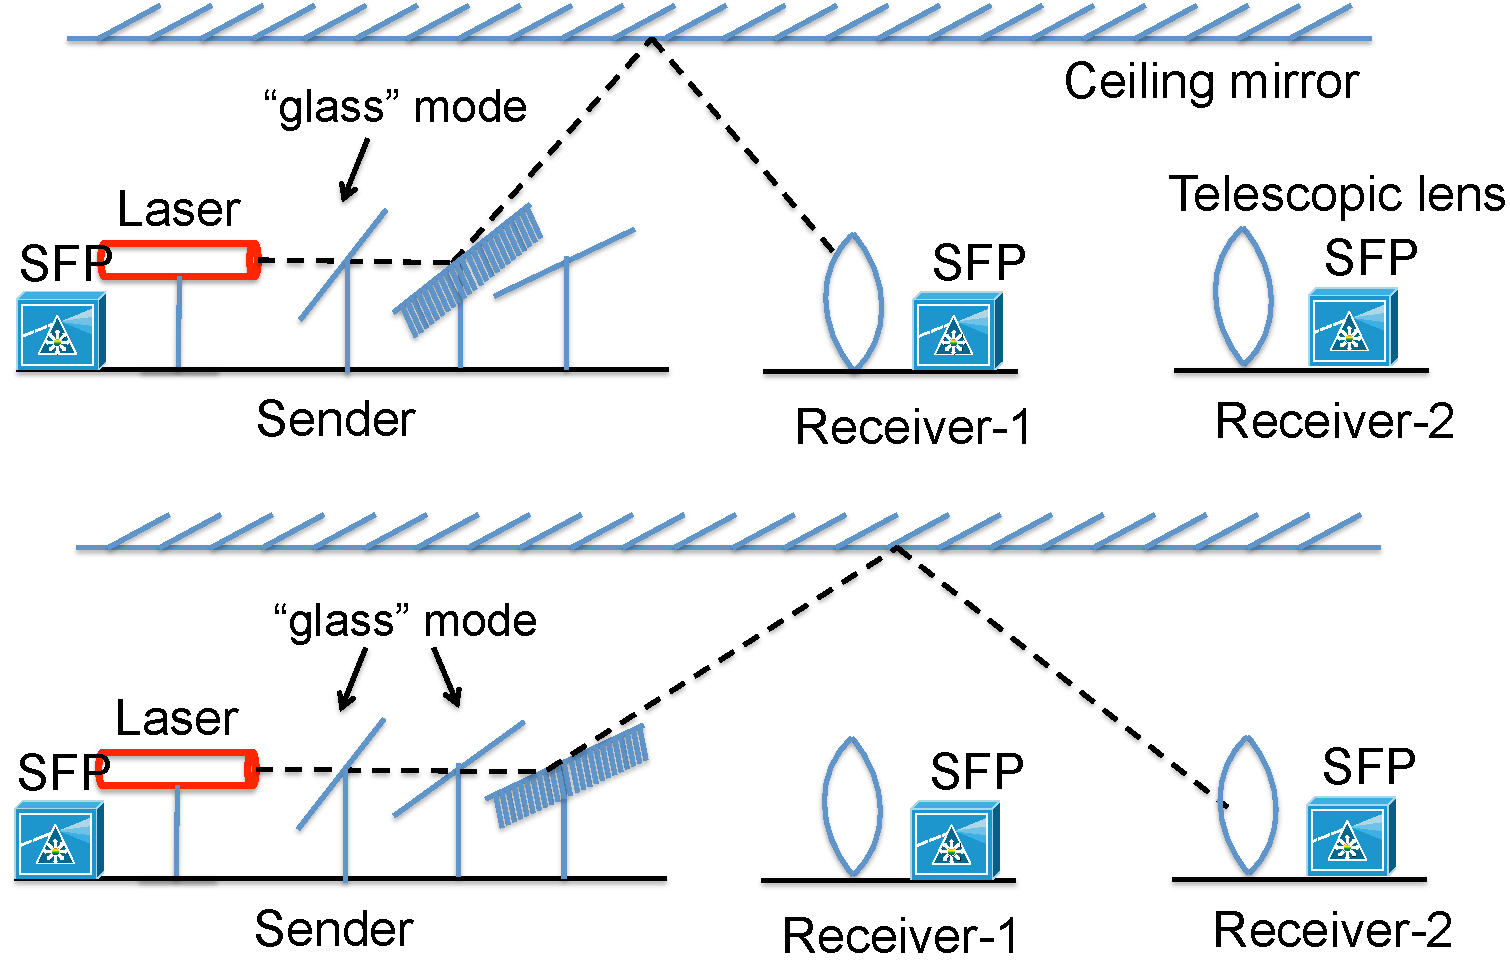
\includegraphics[width=150pt]{Figures/SM-fig.pdf} 
}
\hspace{1cm}
\subfloat[GM: Two mirrors direct incident beam into a rectangular cone. ]
{
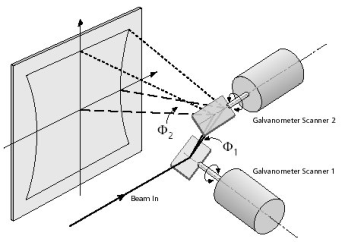
\includegraphics[width=130pt]{Figures/GM-fig.pdf} 
}
\caption{Candidate beam re-direction approaches.}
\label{fig:beam-redirect}
\end{figure*}

%wrapfigure}

%\vyas{why is it called galvo, where was it used before?}

\paragraph*{Galvo Mirrors} A Galvo mirror (GMs)~\cite{} 
is basically a Galvanometer in principle, except
that instead of moving a pointer in response
to current, it moves a small mirror. 
GMs are conventionally 
 used in various laser scanning applications -- both precision industrial as well as infotainment like
 laser shows. 
 As shown  in Figure~\ref{fig:beam-redirect}(b), two computer-controlled, motorized
mirrors are mounted at right angles direct the incident beam into a
rectangular cone.  The (fixed) incident beam can thus be directed into a
rectangular cone under computer control.
   Commercially available
systems~\cite{} can provide a cone half angle ($\Phi_1$ and $\Phi_2$) of
$\pm 20^\circ$, for a total rectangular cone angle of $40^\circ$ in both
directions.  A typical pointing accuracy is within 15 $\mu$rad~\cite{},
resulting in a beam positioning precision within 1.5mm for beam paths of
up to 100m. Typical steering latency is \plsfill. 
\samir{We should say something about MEMS. The reason is that this is something
that an optical net person (typical reviewer) will think first as this is used in optical switches. I think there
was some text in the earlier version. We can put that back in.}

%% TRADEOFF AND PUNT HYBRID
\paragraph*{Tradeoffs}  Use of SM vs. GM present several design tradeoffs. First, use of GM may obviate
the need for additional alignment (e.g., piezo electric positioners). Second,
because of the continuous angle,  it can reach any receiver within the
cone, while SMs  provide a small, discrete number of possibilities.  But the limitation of GM
is that the limited steering angle that makes the
network topology dependent on layout geometry and rack locations. 
Also commodity GM assemblies are much larger than we desire due to the size of 
the motor as well as the driving electronics. One way to reduce the size is to hide the motor
and associated electronics underneath and use custom designed
extension arms to hold the mirrors. But additional stability and precision 
issues must be addressed. This way
only optical components will be present on the top of the rack. 
%
In general,  because the use-cases we envision are significantly beyond the intended
applications of either SM and GM,  we will systematically investigate the impact of these tradeoffs  
and we will likely use a  hybrid
architecture as discussed in Section~\ref{sec:topology}.
\samir{check and make sure we discuss.}

\paragraph*{\Preconfiguration and Overall Cost Issues}
Both SMs and GMs will need to be orientated right so that they can form the desired
set of FSO links. Since this is to be done in a semi-offline fashion, speed
is not of the essence. Also, the actual orientations can be pre-calculated
at the installation time. Orientation can be achieved by servos that simply
orient the attached component (e.g., SM, GM) to a pre-determined position. 
Final corrections are to be done using the piezo electric positioners. 
While we will develop topology design issues for \Preconfiguration 
in Section~\ref{sec:topology},  we consider the actual engineering of this outside
the scope of this project. \samir{We told you how to do this at a high level; don't ask further questions.}

Finally, a word about the cost. As is apparent, our goal is to {\em repurpose
commercially available} components to build the flexible FSO links for \ArchName. 
This is to demonstrate feasibility using current generation technologies. 
However, since the components we will in our actual prototype
are built for different use cases and custom work must be performed, the actual
cost of our prototype (Section~\ref{sec:evalplan}) will exceed expectations by several factors. 
\samir{so that the reviewers do not complain about a link costing ~\$6K.} But 
our back of the envelop calculations show that with a mass-market 
design optimized for the DC, the cost an FSO transceiver including
the steering support will not exceed about \plsfill. \samir{cost is punted.}

%Also,
%existing  GMs are also generally more expensive than SMs and do not
%exist in the small form factors we desire,\vyas{we said nothing about
%cost} To address this concern, we will provide a custom-built GM design
%using \plsfill.
%


% based on the tradeoffs  between cost, degree of reconfigurability,  and form factor.

 



\subsection{Early Demonstration of  Feasibility} % Proof-of-Concept Prototype}

\begin{figure}
%\begin{wrapfigure}{r}{0.8\textwidth}
\vspace{-0.5cm}
\centering
\subfloat[FSO prototype on an optical bench set up]
{
%\vspace{-0.8in}
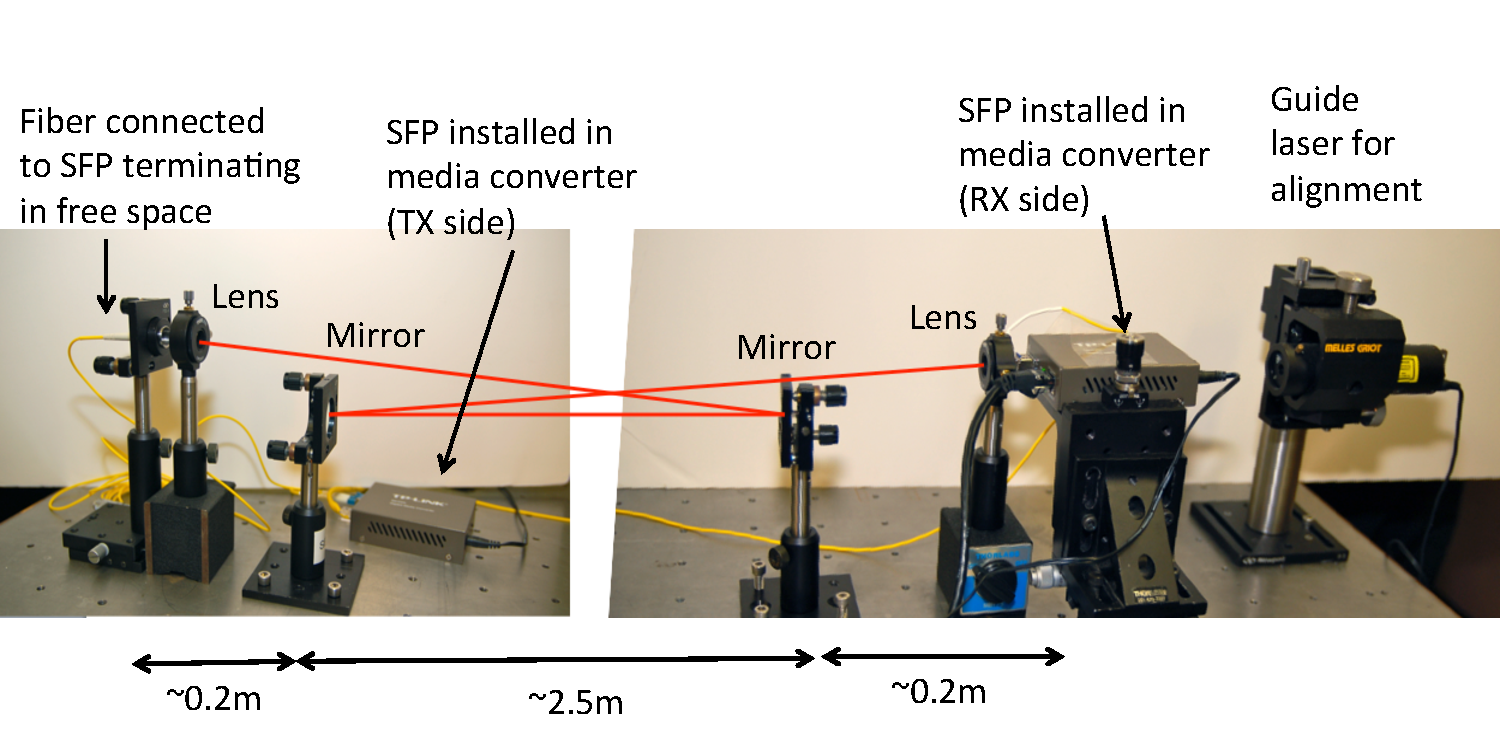
\includegraphics[width=250pt]{PPTFigs/complete-optical-setup-fig.pdf} 
%\vspace{-0.8in}
} 
\hspace*{0.3in}
\subfloat[Throughput stability]
{
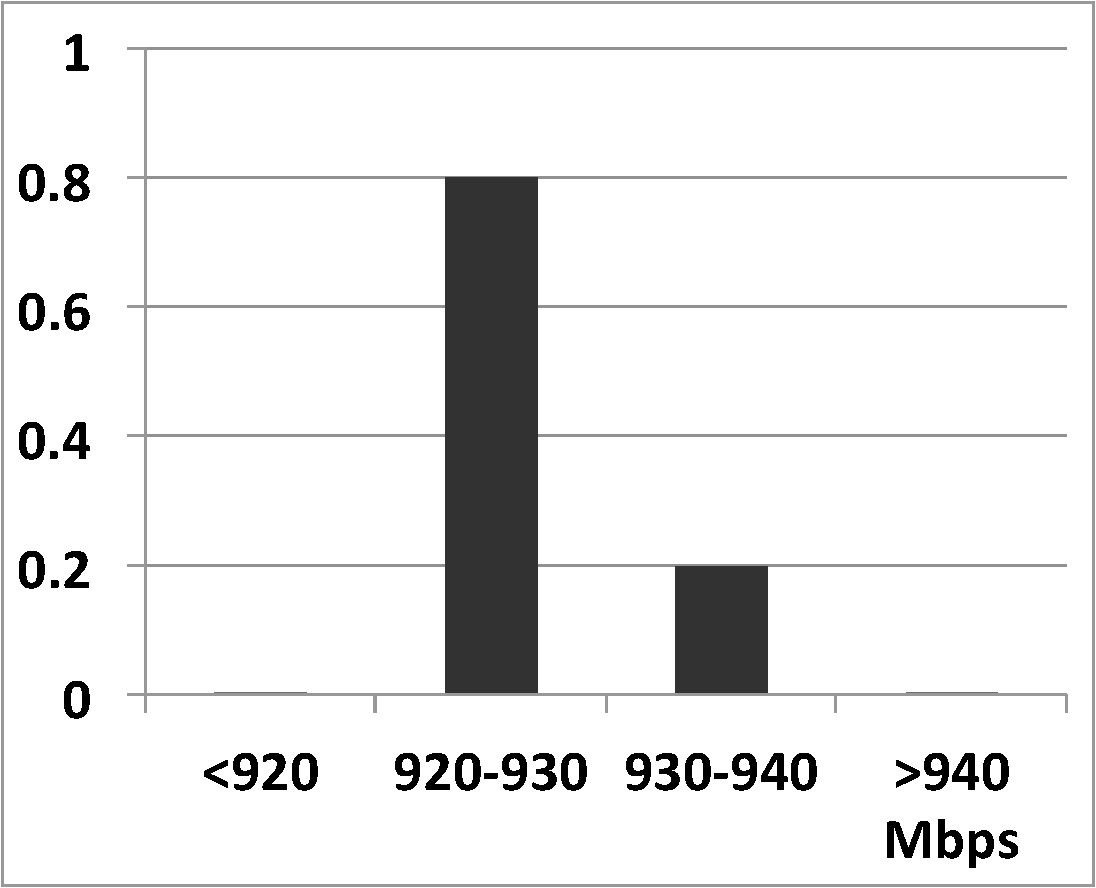
\includegraphics[width=100pt]{Figures/link-thrpt.pdf} 
}
\caption{(a) Experimental prototype showing FSO communication using SFP over ~7.5m.
Note use of mirrors to achieve a long beam path on a standard size optical bench. (The beam is hand drawn.) 
(b) Distribution
of per-second TCP throughputs (in Mbps) over a continuous 30 hour period over ~7.5m.}
\label{fig:optics-layout}
%\end{wrapfigure}
\end{figure}

We developed a proof-of-concept prototype to demonstrate free space
communication using commodity  SFPs shown in 
Figure~\ref{fig:optics-layout}. The prototype uses a pair of  1Gbps SFPs
using 1310nm lasers. % Instead of launching the beam directly from the SFP
 We launch the beam from a single mode optical fiber  connected to the TX
SFP on one end with the other end terminating in free space. Due to the
narrow $8-10 \mu\mbox{m}$ fiber diameter the initial beam divergence is
very large. We used an achromatic doublet lens  to collimate the beam to
a roughly 4mm diameter waist with the fiber tip positioned at the focal
point of the lens. (An optical bench and translating mounts help in the
positioning.) The collimated beam propagates  to a distance of 7.5m
where an identical lens re-focuses beam on the RX detector.\footnote{Since the SFP used here uses two separate optical paths (for duplex
operation), the return link is closed using a regular fiber.}
% This way
%standard network protocols can be run to characterize the free space
%link. 

We connect two laptops to the SFPs via standard media converters~\cite{} and
run TCP throughput experiments for 30 hours to test link stability.
Figure~\ref{fig:optics-layout}  demonstrates very  stable link  performance
comparable to the wired case.  We also analyzed the sensitivitity to
misalignment between the TX-RX and found that the throughput is stable up to a
transverse shift of $\pm0.7$ (not shown).

%addressing alignment issues. Beyond this the throughput drops sharply
%going to zero within another 0.1mm.



We  also independently  evaluated the viability of switchable
mirrors~\cite{hotnets} using a 12" x 15" switchable mirror (SM) from
Kentoptronics~\cite{sm} tuned for the IR spectrum. The switching latency of the
SM is found to be around 250 msec. Because the switching latency is
proportional to the SM’s surface area~\cite{sm-size}, we estimate a $<5$ msec
latency for a small (1" x 1") SM we propose to use. Finally, we confirmed
that the FSO beam can be reflected from conventional mirrors with no loss in
TCP throughput even after multiple reflections. 



